\documentclass[a4paper]{scrreprt}
\usepackage[utf8]{inputenc}
\usepackage{amsmath}
\usepackage{amssymb}
\usepackage{amsopn}
\usepackage{listings}
\usepackage{enumitem}
\usepackage{graphicx}

\newcommand{\norm}[1]{\left\lVert #1 \right\rVert}
\newcommand\ol\overline
\newcommand\N{\mathbb N}
\newcommand\Z{\mathbb Z}
\newcommand\F{\mathbb F}
\DeclareMathOperator{\ess}{ess}
\DeclareMathOperator{\sgn}{sgn}
\DeclareMathOperator{\ord}{ord}
\newcommand{\df}{\mathrm{d}}
\setlength{\parindent}{0em}
\setlength{\parskip}{0.75em}
\renewcommand*{\arraystretch}{1.5}
\renewcommand\mod{\ \mathrm{mod}\:}

\lstset{basicstyle=\small\ttfamily}

\begin{document}

\section*{Exercise 1}

\textbf{Recall.}

\begin{center}
    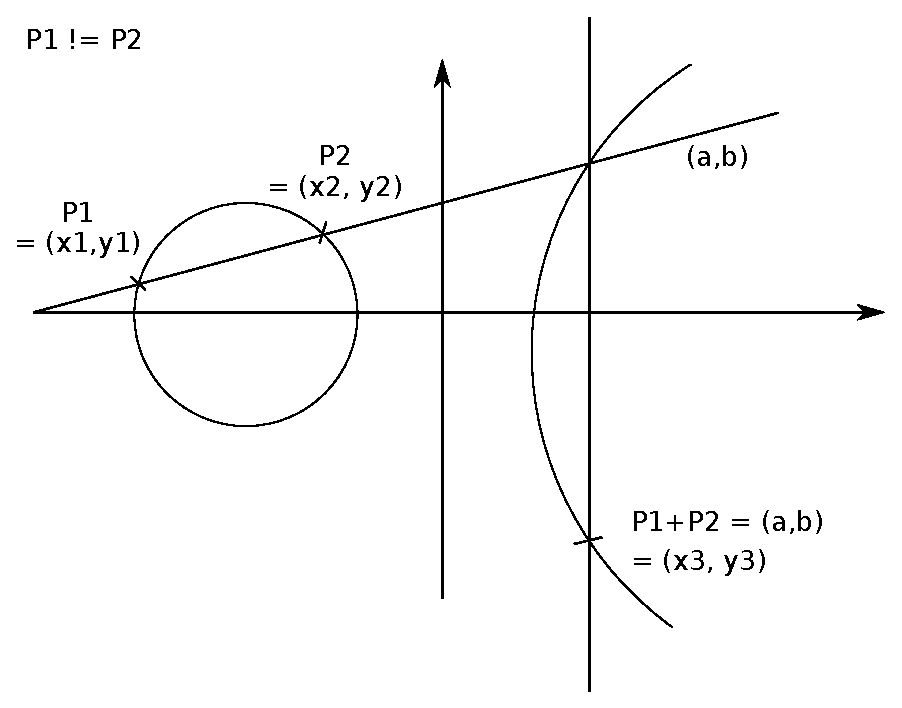
\includegraphics[scale=0.6]{graph1.eps}
\end{center}

\begin{eqnarray*}
    \alpha &=& \frac{y_2-y_1}{x_2-x_1}\\
    x_3 &=& \alpha^2 - x_1 - x_2 \;=\; a \\
    y_3 &=& -y_1+\alpha(x_1-x_3)\;=\;b\\
    E: y^2 &=& x^3 + ax + b
\end{eqnarray*}

\begin{center}
    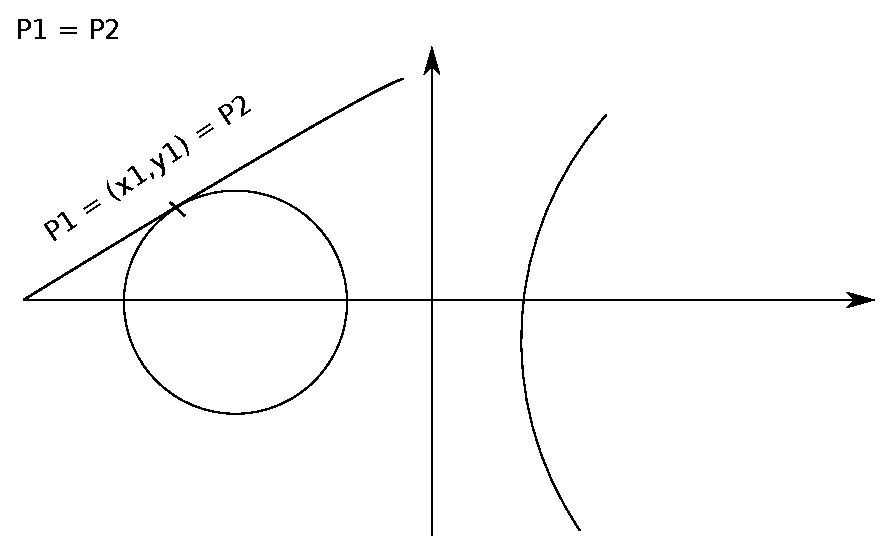
\includegraphics[scale=0.6]{graph2.eps}
\end{center}

\begin{eqnarray*}
    \alpha &=& \frac{dy}{dx} \;=\; \frac{3x_1^2+a}{2y_1}\;=\; \frac{3x_2^2+a}{2y_2}\\
    P_1+P_2 &=& P_3 = 2P_1 = (x_3,y_3)\\
    x_3 &=& \alpha^2 - ??
\end{eqnarray*}

\textit{(Solution Exercise 1 missing)}

\section*{Exercise 2}

Let $n=15$. Write a table of $(\alpha, \alpha^2)$ with $\alpha\in\Z_{15}$.

\begin{center}
    \begin{tabular}{c|c|c|c|c|c|c|c|c|c|c|c|c|c|c|c}
        $\alpha$ & 0 & 1 & 2 & 3 & 4 & 5 & 6 & 7 & 8 & 9 & 10 & 11 & 12 & 13 & 14 \\
        \hline
        $\alpha^2$ & 0 & 1 & 4 & 9 & 1 & 10 & 6 & 4 & 4 & 6 & 10 & 1 & 9 & 4 & 1
    \end{tabular}
\end{center}

Solutions of
\begin{eqnarray*}
    x^2 &\equiv& 0\mod15 \quad x\in\{0\}\\
    x^2 &\equiv& 1\mod15 \quad x\in\{1,4,11,14\}\\
    x^2 &\equiv& 2\mod15 \quad x\in\{\}\\
    x^2 &\equiv& 6\mod15 \quad x\in\{6,9\}\\
\end{eqnarray*}


\section*{Exercise 3}

Suppose $n = 713,\;c = 289$
\[\left\{\begin{array}{ll}
        \sqrt c = 17 \mod n\\
        \sqrt c = 293 \mod n\\
        \sqrt c = 420 \mod n\\
        \sqrt c = 696 \mod n\\
    \end{array}\right.\]

Find the factorization of $n$.

\begin{eqnarray*}
    \gcd(293-17, n) &=& 23 \\
    \gcd(293-420, n) &=& 1 \\
    \gcd(293 - 696, n) &=& ?
\end{eqnarray*}

$n = 713 = 23 \cdot 31$.

\section*{Exercise 4}

Let $p=19$.

Square table of $\Z_p$:
\vspace*{-1em}
\begin{center}
    \begin{tabular}{c|c|c|c|c|c|c|c|c|c|c|c|c|c|c|c|c|c|c|c}
        $\alpha$ & 0 & 1 & 2 & 3 & 4 & 5 & 6 & 7 & 8 & 9 & 10 & 11 & 12 & 13 & 14 & 15 & 16 & 17 & 18\\
        \hline
        $\alpha^2$ & 0 & 1 & 4 & 9 & 16 & 6 & 17 & 11 & 7 & 5 & 5 & 7 & 11 & 17 & 6 & 16 & 9 & 4 & 1\\
    \end{tabular}
\end{center}

Square root map of $\Z_p$:
\[\mathit{Sqrt}: \{0,1,4,5,7,9,11,16,17\}\rightarrow\Z_{19}\]
\[\beta\mapsto\mathit{Sqrt}(\beta)=\beta^{\frac{q+1}2}=\beta^5\]
where $2q=p+1$.

Square root table:
\vspace*{-1em}
\begin{center}
    \begin{tabular}{c|c|c|c|c|c|c|c|c|c|c}
        $\beta$ & 0 & 1 & 4 & 5 & 6 & 7 & 9 & 11 & 16 & 17\\
        \hline
        $\sqrt\beta$ & $0^5$ & $1^5$ & $4^5$ & $5^5$ & $6^5$ & $7^5$ & $9^5$ & $11^5$ & $16^5$ & $17^5$ \\
        $\mathit{Sqrt}(\beta)$ & 0 & 1 & 17 & 9 & 5 & 11 & 16 & 7 & 4 & 6
    \end{tabular}
\end{center}

\section*{Exercise 5}

$(b_1): (182,637,92,275,368,373,109,491),\;m=1000,\;c=678,\;\lambda=91$
\begin{eqnarray*}
    \lambda^-{-1}\mod m &=& 91^{-1}\mod 1000\;=\;11\\
    \lambda^-{-1}\cdot c &=& 11\cdot678\;=\;458\;=\;c'\\
\end{eqnarray*}
\[lambda^-{-1}\cdot(b_1) : (2,7,12,25,48,103,199,401)\]
\[c'=458=401+48+7+2\] thus \[c=678=182+637+368+491\mod m\]
\[m=(1,1,0,0,1,0,0,1)\]

\end{document}

